%\renewcommand{\theequation}{\theenumi}
%\begin{enumerate}[label=\thesubsection.\arabic*.,ref=\thesubsection.\theenumi]
%%\begin{enumerate}[label=\arabic*.,ref=\thesection.\theenumi]
%\renewcommand{\thefigure}{\theenumi}    
%\numberwithin{equation}{enumi}
% \numberwithin{equation}{enumi}
% \numberwithin{figure}{enumi}
% \numberwithin{table}{enumi}



\item Construct $\triangle PQR$, given that $PQ = 3, QR = 5.5$ and $\angle PQR = 60 \degree$.
\\
\solution
\begin{align}
    \because \vec{P} = r\myvec{\cos Q\\ \sin Q}, \vec{Q} = \myvec{0\\0}, \vec{R} = \myvec{p\\0}
    \end{align}
    from the given information, 
    \begin{align}
    \vec{P} = 3\myvec{\cos60\\ \sin60} = \frac{3}{2}\myvec{1\\\sqrt3},  \vec{Q} = \myvec{0\\0},  \vec{R} = \myvec{5.5\\0}
    \end{align}
and plotted in Fig.              \ref{constr/july/1Figure}.
    
    
\begin{figure}[!ht]
\centering
         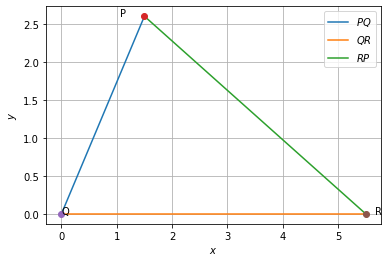
\includegraphics[width= \columnwidth]{solutions/july/2/1/figure1.png}
         \caption{The Constructed triangle}
         \label{constr/july/1Figure}
\end{figure}






%
\item Construct $\triangle ABC$  with $BC = 7.5, AC = 5$ and $\angle C = 60\degree$.
\\
\solution

\begin{align}
\because     \vec{A} = b\myvec{\cos C\\ \sin C}, \vec{B} = \myvec{a\\0}, \vec{C} = \myvec{0\\0},
    \end{align}
    substituting the given values, 
    \begin{align}
        \vec{A} = 5\myvec{\cos60\\ \sin60} = \myvec{2.5\\2.5\sqrt3},  \vec{B} = \myvec{7.5\\0},  \vec{C} = \myvec{0\\0}
        \end{align}
    which are plotted in Fig. \ref{constr/july/2Figure}.       

\begin{figure}[!h]
         \centering
         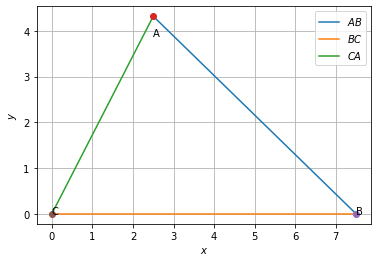
\includegraphics[width= \columnwidth]{solutions/july/2/2/Figures/Figure 1.png}
         \caption{The Constructed triangle}
         \label{constr/july/2Figure}
\end{figure}




\item Construct $\triangle XYZ$ if $XY = 6, \angle X = 30\degree$ and $\angle Y = 100 \degree$.
\item If $AC = 7, \angle A = 60\degree$ and $\angle B = 50 \degree$, can you draw the triangle?
%
\solution
\input{}

\item Construct $\triangle PQR$ if $PQ = 5, \angle Q = 105 \degree$ and $\angle R = 40 \degree$.
\item Can you construct $\triangle DEF$ such that $EF = 7.2, \angle E = 110\degree$ and $\angle F = 180\degree$?
\item Construct the  triangles in Table \ref{table:triangle_const_exercises}.
\begin{table}[!ht]
\centering
\input{./chapters/constr/Triangle}
\caption{}
\label{table:triangle_const_exercises}
\end{table}
\solution
\begin{enumerate}
    \item
    \item 
    \solution
    We obtain the vertices of the rhombus as follows
\begin{align}
\vec{A} = \myvec{-3\\0},
\vec{B} = \myvec{0\\-3.5},
\vec{C} = \myvec{3\\0},
\vec{D} = \myvec{0\\3.5}
\end{align}
which are plotted in Fig. \ref{quad/45/fig:Rhombus ABCD}.
%
\begin{figure}[ht!]
\centering
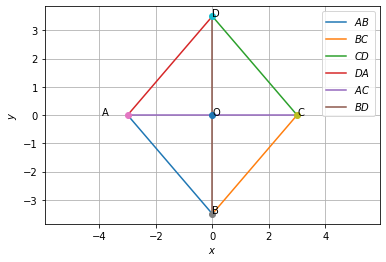
\includegraphics[width=\columnwidth]{solutions/quad/45/figure2.png}
\caption{Rhombus ABCD}
\label{quad/45/fig:Rhombus ABCD}
\end{figure}

    \item 
    \solution
    From the given information,
%
\begin{align}
\angle{C} = \ang{60}
\end{align}
%
Using the sine formula, 
%
\begin{align}
c &= b \brak{\frac{\sin{C}}{\sin{B}}} 
\\
&= 3.3915
\end{align}
%
the vertices of $\triangle ABC$ are
\begin{align}
\vec{A} = \myvec{0 \\ 0},
\vec{B} = c\myvec{\cos{\ang{70}} \\ \sin{\ang{70}}},
\vec{C} = \myvec{3 \\ 0}
\end{align}
and  plotted in Fig. \ref{constr/tri/27/3/fig:triangle ABC}.
%
\begin{figure}[ht]
    \centering
    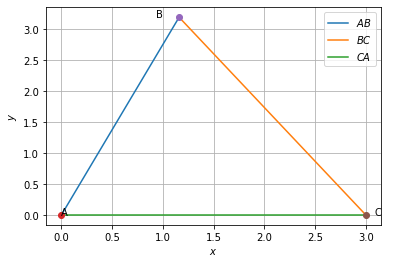
\includegraphics[width=\columnwidth]{solutions/triangle/27/3/Triangle_ABC.PNG}
    \caption{Plot of $\triangle ABC$}
    \label{constr/tri/27/3/fig:triangle ABC}
\end{figure}


        
\end{enumerate}
%
